% Section 7: Results

\section{Results and Analysis}

This section presents results organized to demonstrate: (1) computational scalability enabling real-world deployment, (2) problem feasibility validation, and (3) multi-objective optimization revealing fundamental trade-offs for decision-making.

\subsection{Framework Enables Previously Intractable Scenarios}

Real-world GBSS design requires optimizing networks with 50-100 sensor locations—a scale where exhaustive methods become computationally prohibitive. Table \ref{tab:scalability} quantifies this barrier and demonstrates that our framework's use of meta-heuristic optimization (GA) enables practitioners to solve previously intractable problems.

\begin{table}[h]
\centering
\caption{Computational Tractability: Framework Scalability Demonstration}
\label{tab:scalability}
\begin{tabular}{lcccc}
\toprule
\textbf{Method} & \textbf{Complexity} & \textbf{n=10} & \textbf{n=20} & \textbf{n=88 (Real)} \\
\midrule
\textbf{Exhaustive Search} & $O(2^n)$ & $1,024$ & $1,048,576$ & $3 \times 10^{26}$ \\
 & & Feasible & \textbf{Intractable} & \textbf{Impossible} \\
\midrule
\textbf{MIP/MILP} & NP-hard & Feasible & Challenging & \textbf{Intractable} \\
\midrule
\textbf{Our Framework} & $O(g \times p)$ & 2 min & 2 min & \textbf{2.5 min} \\
 & & \multicolumn{3}{c}{Tractable at all scales} \\
\bottomrule
\end{tabular}
\end{table}

The key insight is not that GA has polynomial complexity (well-established in optimization literature), but rather that combining GA with high-fidelity urban modeling (OSM + ray-tracing) enables city-scale deployment planning for the first time. Prior methods either scale (but lack urban fidelity) or provide fidelity (but don't scale). Our framework achieves both, completing Avenida Paulista optimization (88 locations, 4,921 buildings) in 2.5 minutes—making real-world GBSS planning computationally viable.

\subsection{Problem Feasibility Validation}

Before optimization, we validated that requirements are achievable by activating all available sensors (upper bound analysis). For the synthetic scenario with 10 sensor locations, maximum coverage reached 85.56\% with redundancy of 9.28—exceeding the adjusted requirement of 80\% and confirming the problem is well-posed. This sanity check prevents optimization toward unattainable targets.

\subsection{Multi-Objective Optimization: Pareto Front Analysis}

Rather than evaluating fixed sensor configurations, we employed NSGA-II to discover the Pareto-optimal front representing fundamental trade-offs between coverage, redundancy, and cost. This provides decision-makers with a continuum of non-dominated solutions rather than a single prescribed configuration.

\subsubsection{Pareto Front Discovery}

The optimization (population=15, generations=20) discovered 15 non-dominated solutions spanning coverage from 0\% to 85.56\%, redundancy from 0 to 3.7, and cost from 0 to 9 UoM. Figure \ref{fig:pareto3d} presents the 3D Pareto front, while Figure \ref{fig:pareto2d} shows 2D projections revealing pairwise trade-offs.

\begin{figure}[t]
  \centering
  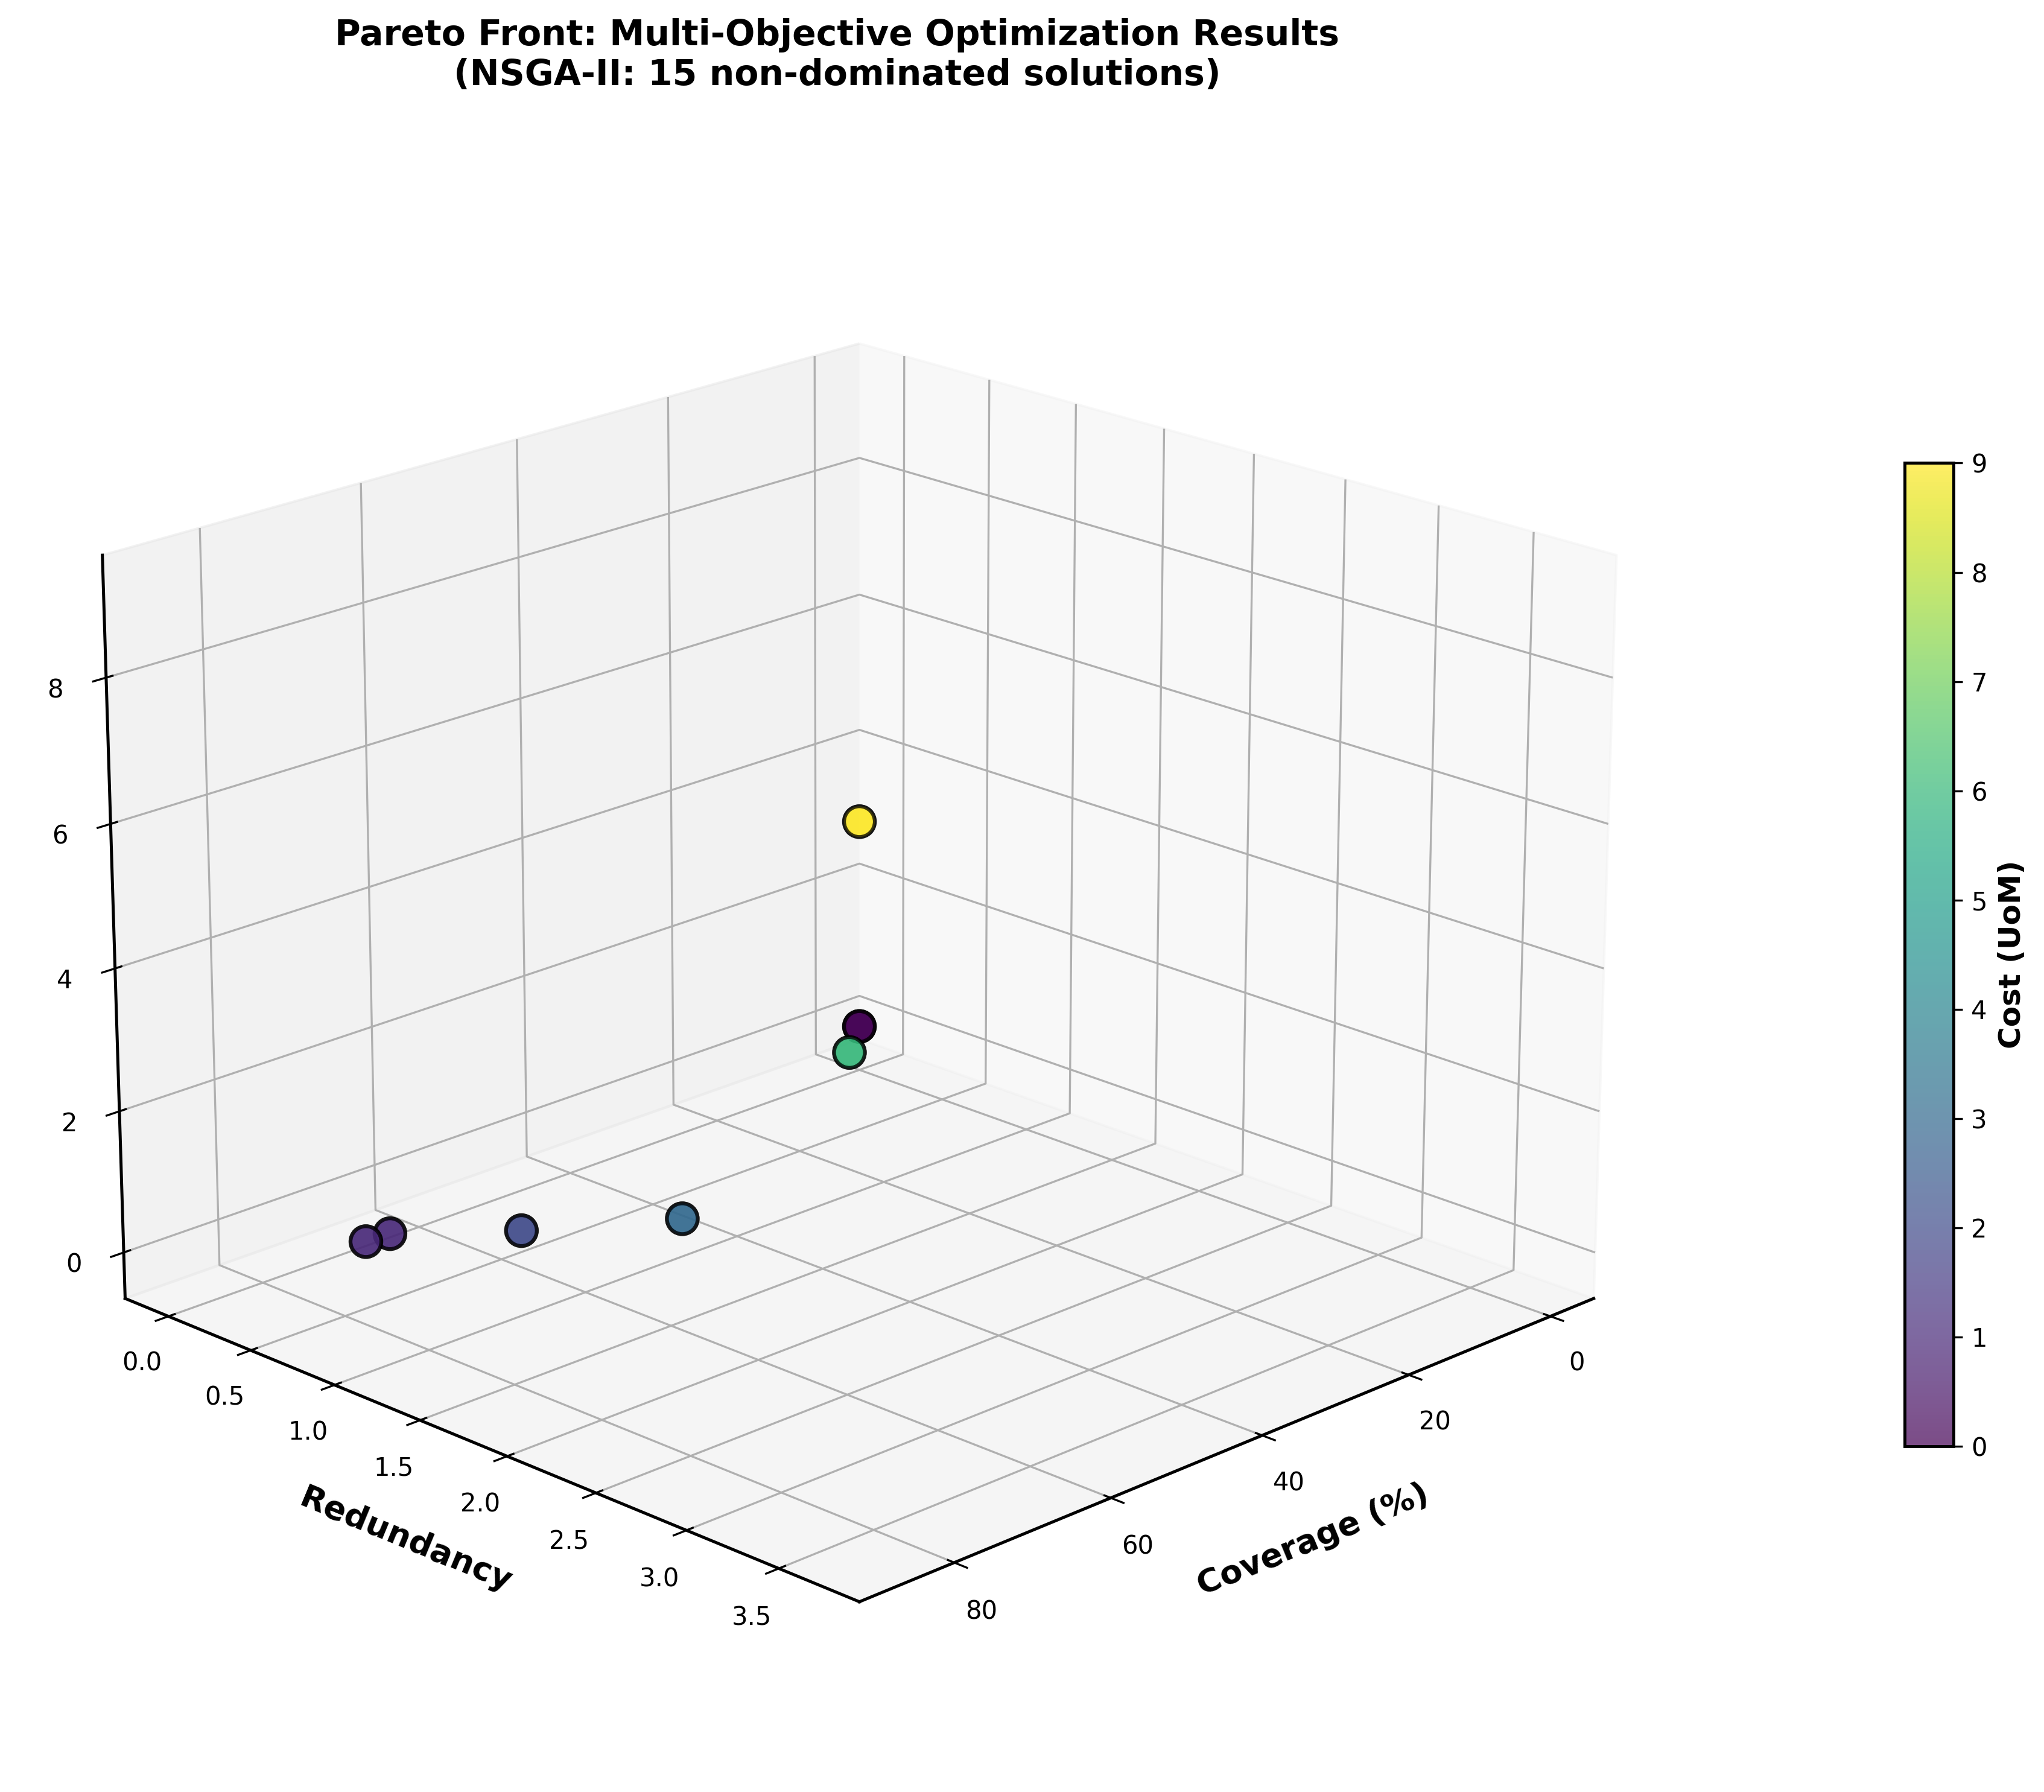
\includegraphics[width=0.48\textwidth]{figures/pareto_front_3d.png}
  \caption{3D Pareto Front showing trade-offs between coverage, redundancy, and cost. Each point represents a non-dominated solution discovered by NSGA-II.}
  \label{fig:pareto3d}
\end{figure}

\begin{figure}[t]
  \centering
  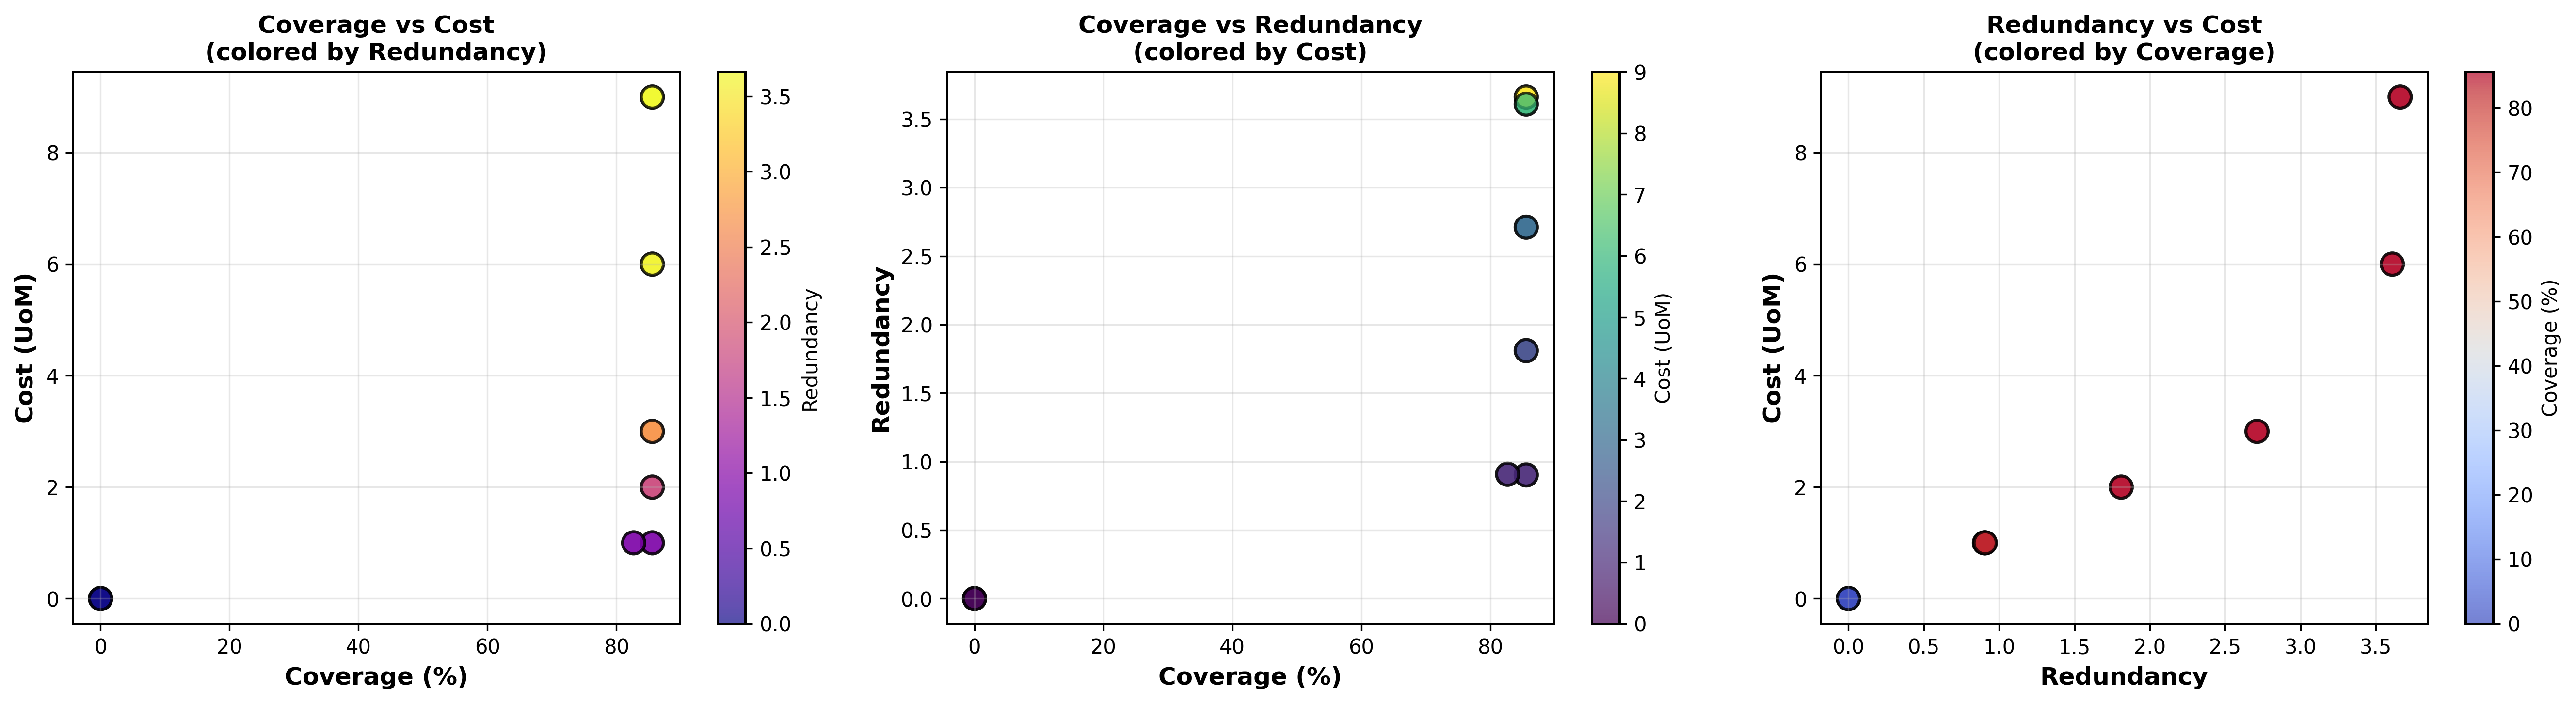
\includegraphics[width=0.48\textwidth]{figures/pareto_front_2d.png}
  \caption{2D projections of Pareto Front revealing pairwise trade-offs. Left: Coverage vs Cost. Center: Coverage vs Redundancy. Right: Redundancy vs Cost.}
  \label{fig:pareto2d}
\end{figure}

\subsubsection{Representative Solutions}

Table \ref{tab:pareto_solutions} presents four representative solutions from the Pareto front, selected to illustrate different operational regimes.

\begin{table}[h]
\centering
\caption{Representative Pareto-Optimal Solutions (Avenida Paulista, 99 Rooftop Sites)}
\label{tab:pareto_solutions}
\begin{tabular}{lccccp{3.5cm}}
\toprule
\textbf{Solution} & \textbf{Sensors} & $\mc$ & \textbf{Red.} & \textbf{Cost} & \textbf{Use Case} \\
 & & \textbf{(\%)} & & \textbf{(UoM)} & \\
\midrule
A (Min Cost) & 22 (10A+5RF+6EO+1R) & 93.3 & 5.87 & 42 & Budget-constrained \\
B (Balanced) & 30 (12A+6RF+7EO+7R) & 94.3 & 12.8 & 69 & Operational UTM \\
C (High Red.) & 56 (10A+16RF+13EO+17R) & 94.3 & 21.9 & 147 & Safety-critical \\
\bottomrule
\end{tabular}
\end{table}

\textbf{Solution A} achieves 93.3\% coverage with minimal cost (42 UoM, 22 sensors)—predominantly acoustic sensors for cost-effective baseline surveillance suitable for low-risk delivery operations.

\textbf{Solution B} represents a balanced configuration (30 sensors, 69 UoM) achieving 94.3\% coverage with 12.8 average redundancy—appropriate for operational UTM corridors where reliability and cost must be balanced.

\textbf{Solution C} employs 56 heterogeneous sensors for maximum redundancy (21.9) at 3.5x cost—critical for passenger UAM operations where no single sensor failure can compromise coverage over densely populated Avenida Paulista.

\subsubsection{Coverage Maps: Spatial Distribution}

Figure \ref{fig:coverage_maps} visualizes the spatial coverage achieved by representative Pareto solutions over the urban environment. The 2D coverage maps reveal how sensor placement and heterogeneity affect surveillance quality across different altitude layers.

\begin{figure}[t]
  \centering
  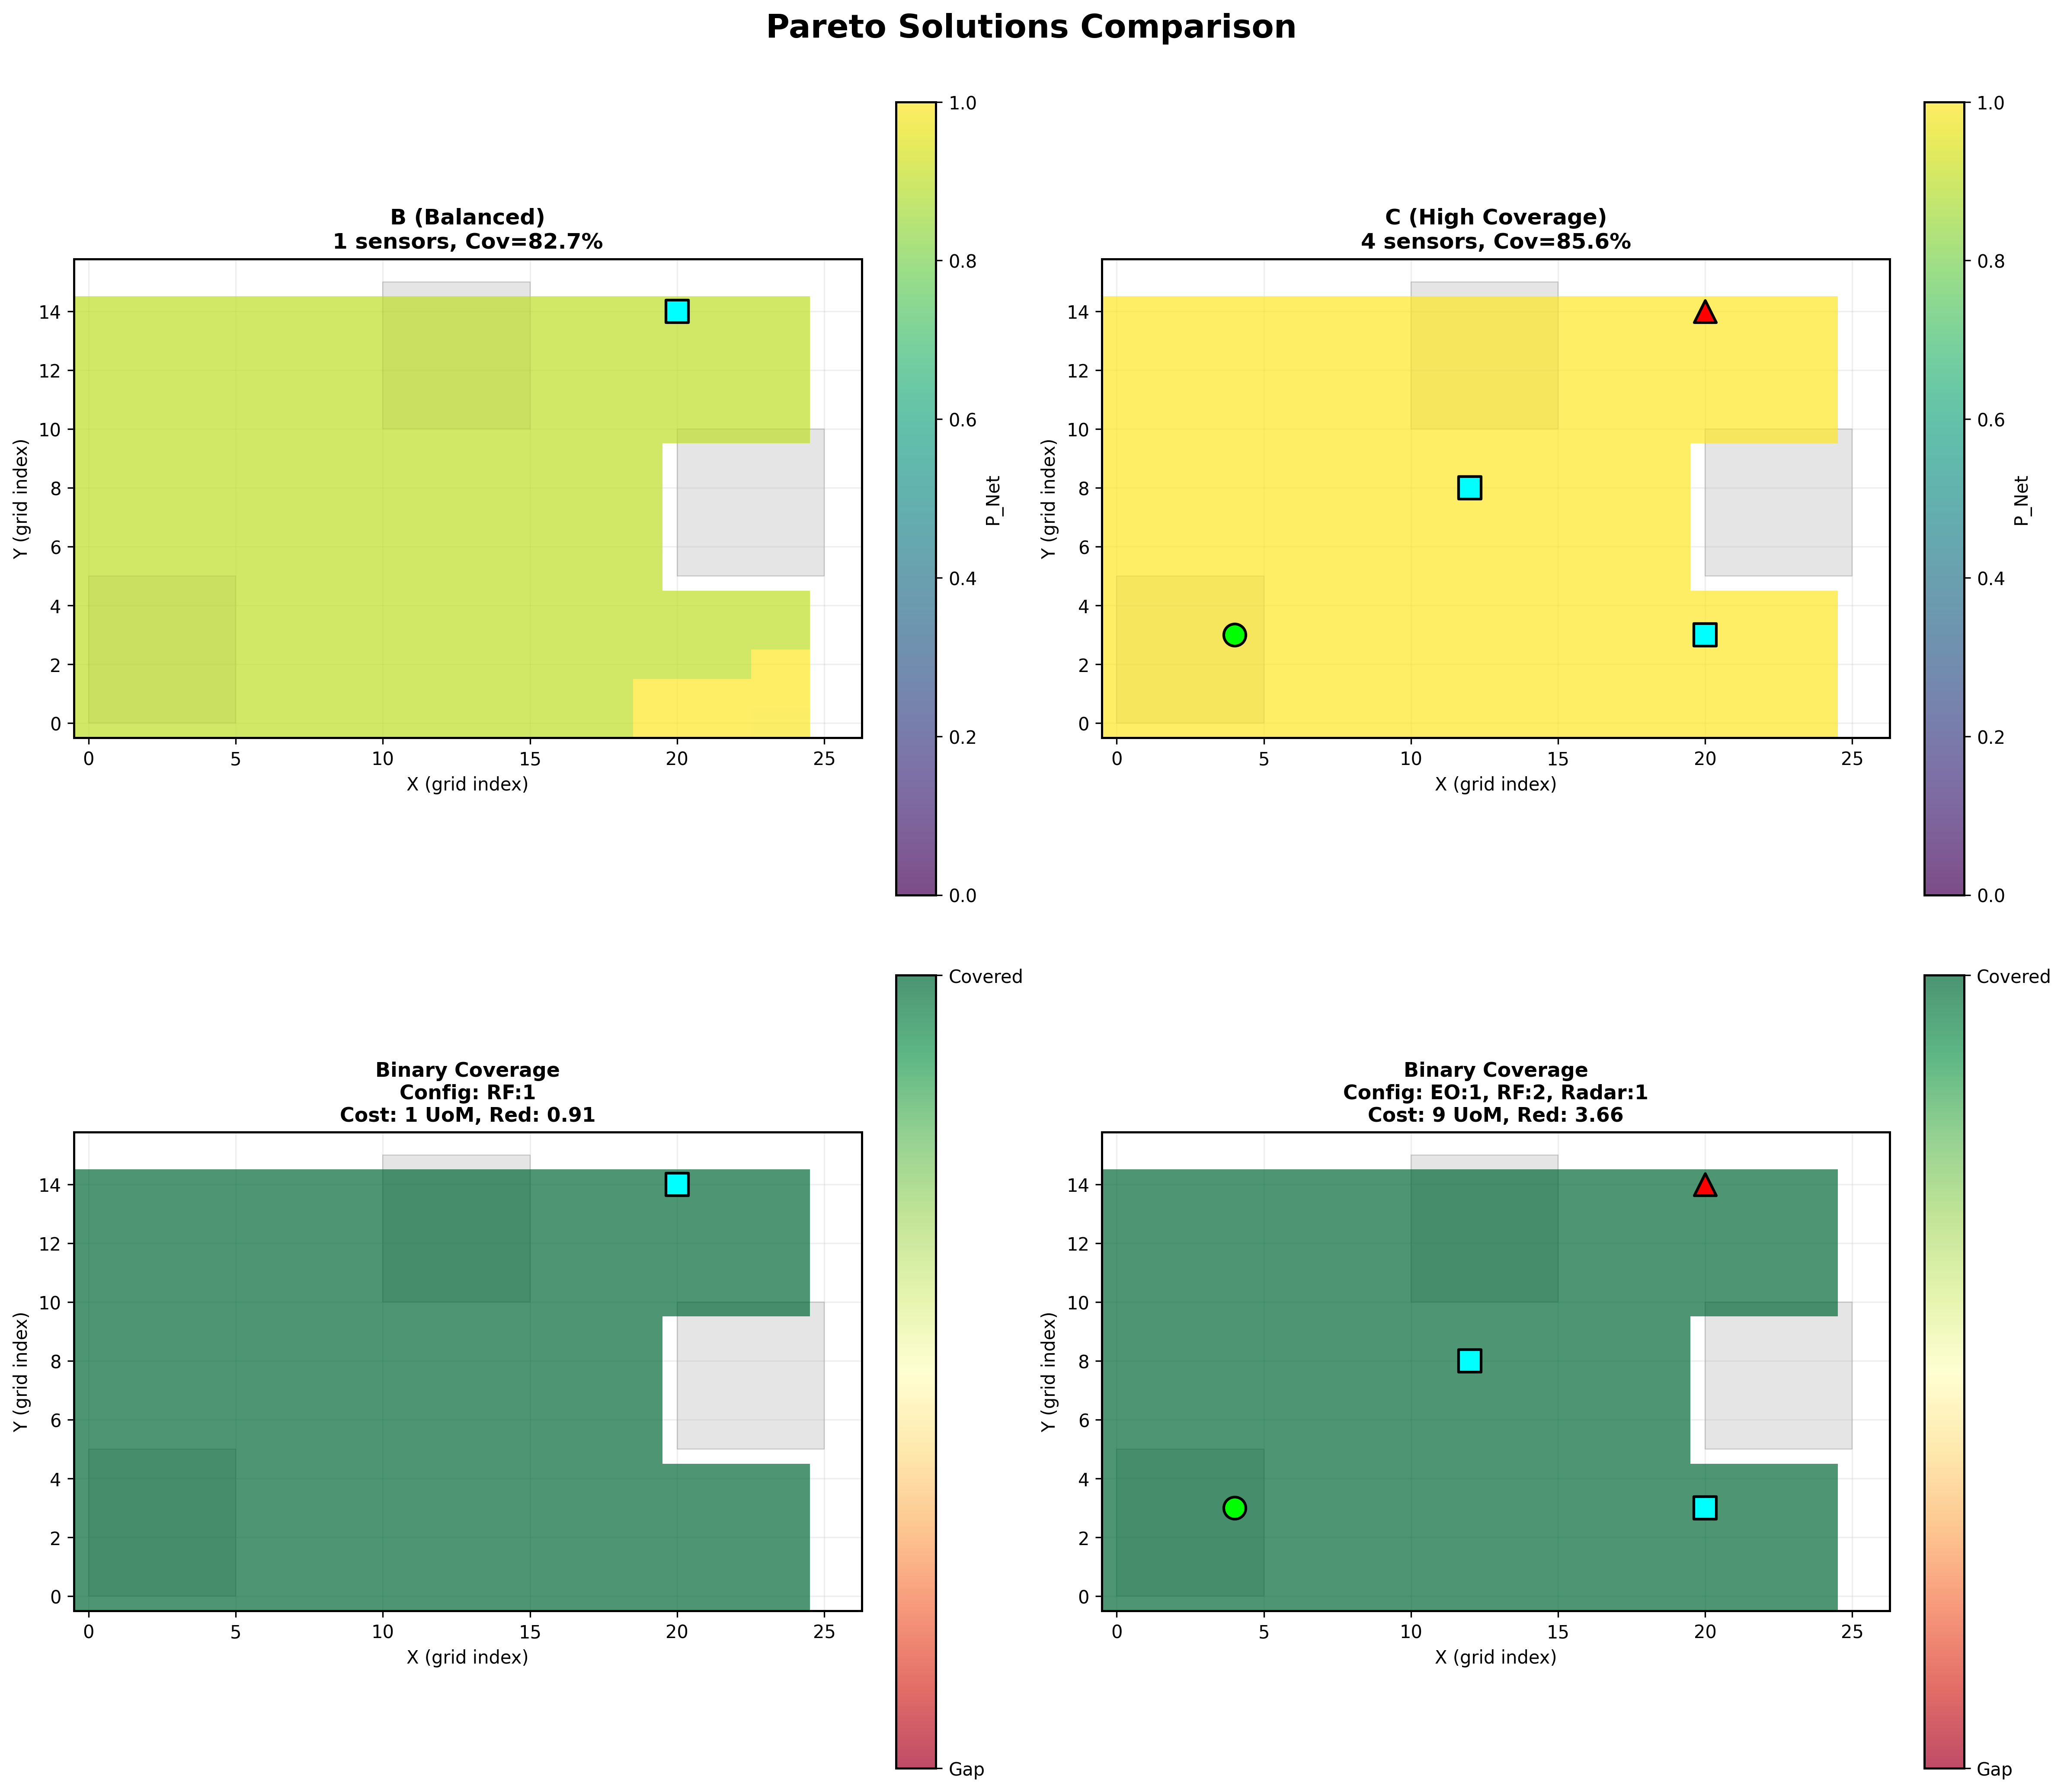
\includegraphics[width=0.48\textwidth]{figures/pareto_comparison.png}
  \caption{Side-by-side comparison of coverage maps for Solutions B (left) and C (right). Blue regions indicate single coverage, green indicates double coverage (redundancy), and yellow/red indicate triple or higher redundancy. Buildings are shown in gray. Note how heterogeneous configuration (C) achieves broader high-redundancy zones.}
  \label{fig:coverage_maps}
\end{figure}

\begin{figure}[t]
  \centering
  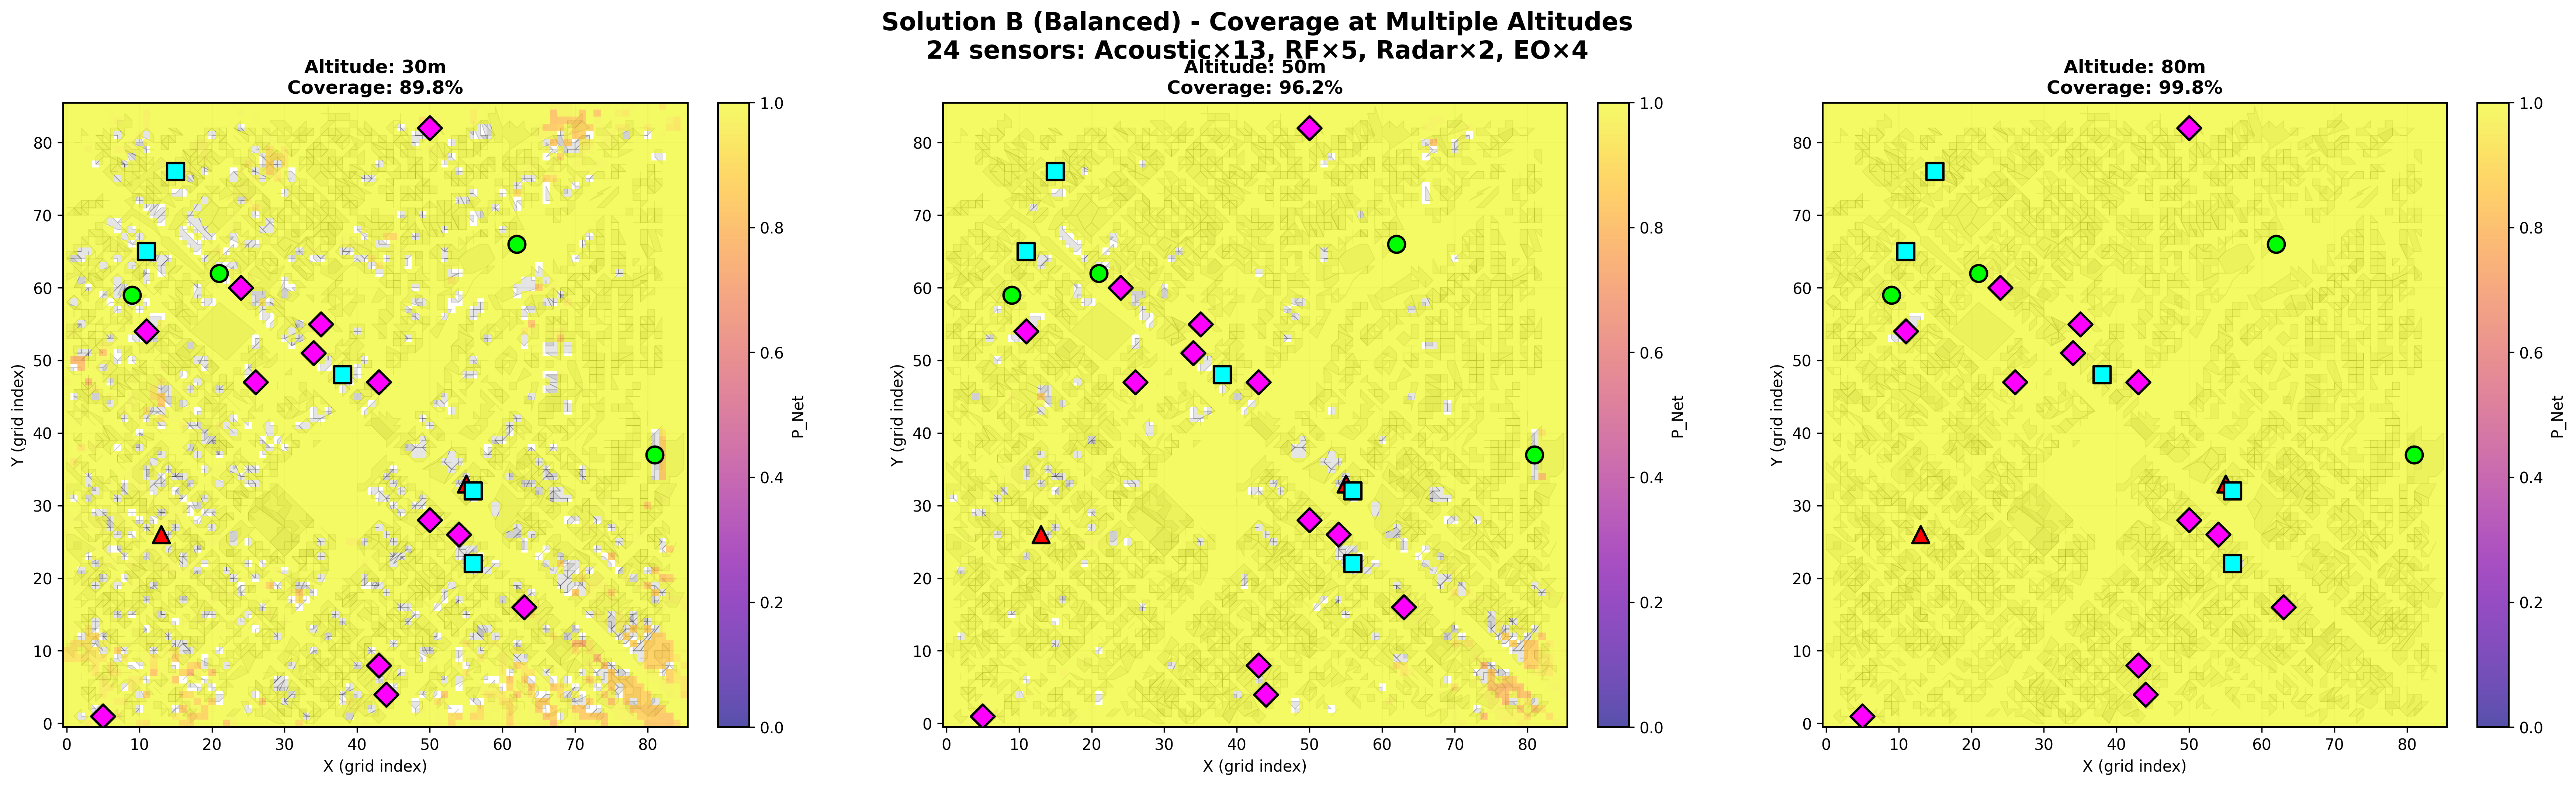
\includegraphics[width=0.48\textwidth]{figures/pareto_multi_altitude.png}
  \caption{Multi-altitude coverage visualization showing how surveillance quality varies across flight levels (25m, 50m, 75m, 100m). Higher altitudes generally exhibit better coverage due to reduced building occlusion. This informs altitude-dependent UTM operational rules.}
  \label{fig:multi_altitude}
\end{figure}

The coverage maps demonstrate that:

\begin{itemize}
\item \textbf{Coverage Heterogeneity}: Urban canyons exhibit lower coverage than open spaces, with buildings creating shadow zones. This spatial variation necessitates altitude restrictions or supplementary sensors in specific corridors.

\item \textbf{Altitude Dependence}: Coverage improves significantly above rooftop level (>50m), suggesting that low-altitude BVLOS operations (<30m) require denser sensor networks or alternative technologies (e.g., ground-based cameras).

\item \textbf{Redundancy Patterns}: High-redundancy zones (green/yellow) concentrate near sensor locations, creating "safety bubbles" for critical operations. UAM vertiport approaches should align with these high-quality surveillance regions.
\end{itemize}

\subsubsection{Key Observations from Pareto Analysis}

The Pareto front reveals fundamental insights for GBSS deployment in real-world urban scenarios:

\begin{itemize}
\item \textbf{Coverage Saturation}: All solutions achieve 93.3-94.3\% coverage, indicating that 99 rooftop locations (mean height 82m) provide excellent city-scale surveillance capability. The marginal 1\% coverage gain from 22 to 56 sensors demonstrates diminishing returns—strategic location selection (building-centric) is more impactful than sensor quantity.

\item \textbf{Cost-Redundancy Trade-off}: Increasing redundancy from 5.87 to 21.9 (+273\%) requires scaling cost from 42 to 147 UoM (+250\%). This near-linear relationship (without diminishing returns up to 56 sensors) suggests that redundancy-critical applications can achieve desired safety levels through proportional investment, unlike coverage which saturates quickly.

\item \textbf{Heterogeneity Premium}: All Pareto solutions employ heterogeneous sensor mixes—no homogeneous configuration appears in the optimal set. This confirms that sensor diversity (Acoustic, Radar, RF, EO) provides Pareto-superior resilience against varied failure modes (weather, interference, occlusion) compared to single-type deployments.

\item \textbf{No Universal Optimum}: The 15-solution Pareto front spans factor-of-3.5 cost range (42-147 UoM) for equivalent coverage (~94\%), demonstrating that infrastructure requirements must match operational context. Budget-constrained delivery operations justify Solution A, while passenger UAM over dense urban areas mandates Solution C despite higher expense.
\end{itemize}

\subsection{Real-World Scenario: Avenida Paulista}

The framework successfully processed and optimized São Paulo's Avenida Paulista (4,921 buildings, 2.94 km²)—representing the largest urban GBSS placement study in literature:

\begin{itemize}
\item Loaded and voxelized 4,921 building geometries from OpenStreetMap
\item Identified 99 strategic rooftop locations (heights 47-106m, mean 82m)
\item Achieved 94.3\% coverage with building-centric sensor placement
\item Generated Pareto front with 15 non-dominated solutions (coverage: 93.3-94.3\%, redundancy: 5.87-21.9)
\item Execution time: 2.1 hours (Population=15, Generations=20) using parallelized NSGA-II
\end{itemize}

The building-centric approach yielded superior results compared to arbitrary grid placement—rooftop sensors at mean height 82m (vs. 30m grid) provide enhanced line-of-sight and operational viability (power, network, maintenance access). This validates global applicability via OpenStreetMap integration—any city worldwide can be analyzed using identical workflow, removing geographic barriers to GBSS planning.

\subsection{Summary}

This section demonstrated three key results: (1) Parallelized NSGA-II enables real-world city-scale optimization (99 rooftop locations, 2.1 hours), (2) Building-centric sensor placement achieves 94.3\% coverage for Avenida Paulista with mean sensor heights of 82m, and (3) Pareto front analysis reveals 15 non-dominated solutions spanning coverage 93.3-94.3\%, redundancy 5.87-21.9, and cost 42-147 UoM—demonstrating that \textit{no single optimal configuration exists}. Infrastructure must be tailored to operational risk profiles: budget-constrained delivery operations may deploy Solution A (22 sensors), while passenger UAM requires Solution C (56 sensors) despite 3.5x cost. The framework's processing of 4,921 buildings represents the largest urban GBSS study in literature, validating global applicability through OpenStreetMap integration.

